\documentclass[unicode,11pt]{beamer}
\usetheme{metropolis}
\usefonttheme{professionalfonts}

\usepackage[japanese]{babel}
\usepackage{unicode-math}
\usepackage[no-math,match,deluxe]{luatexja-fontspec}

\usepackage{mathtools,amssymb,amsthm}
\usepackage{multicol}
\usepackage{cleveref}
\usepackage{listings}
\usepackage{pgfplots}
\usepackage{tcolorbox}
\usepackage{xparse}
\usepackage{bxghost}
\usepackage{mathpunctspace}
\usepackage[ISO]{diffcoeff}
\usepackage{cancel}
\usepackage{siunitx}
\usepackage{comment}

% パッケージの初期設定
\usetikzlibrary{cd,arrows.meta}
\tcbuselibrary{xparse,listings,theorems,breakable,skins}
\pgfplotsset{width=7cm,compat=1.18}
\setlength{\columnseprule}{0.4pt}

% メタデータ
\title{直感重視の音声分析入門}
\author{@cuttlefish\_math}
\date{\today}
\institute{基幹理工学部 応用数理学科 2年}

% フォント設定
\setmainjfont{Mplus 1p Regular}[BoldFont={Mplus 1p Medium}]
\setsansjfont{Mplus 1p Regular}[BoldFont={Mplus 1p Medium}]
\setmathfont{Latin Modern Math}

% 参照
\crefname{equation}{式}{式}

% 定理環境
\newenvironment{question}{\begin{block}{\usebeamercolor[fg]{example text} Question}}{\end{block}}
\newenvironment{answer}{\begin{block}{\usebeamercolor[fg]{example text} Answer}}{\end{block}}

% 引用
\definecolor{quotebar}{HTML}{6E7B7E}
\definecolor{quotetext}{HTML}{6E7B7E}

\newenvironment{redditquote}{\begingroup\color{quotetext}}{\endgroup}

\tcolorboxenvironment{redditquote}{%
  blanker,
  before skip=1\zh,
  after skip=1\zh,
  left=15pt,
  borderline west={3pt}{0pt}{quotebar}}

% ソースコード
\definecolor{codeback}{HTML}{EEEEEE}

\lstdefinestyle{codeblock}{%
  aboveskip=0pt,
  belowskip=0pt,
  breaklines=true,
  breakindent=10pt,
  basicstyle=\ttfamily\footnotesize}

\newtcblisting{codeblock}{%
  listing only,
  listing options={style=codeblock},
  enhanced,
  breakable,
  colback=codeback,
  arc=0mm,
  boxrule=0mm,
  top=2mm,
  bottom=2mm,
  left=2mm,
  right=2mm,
  frame hidden}

\NewDocumentCommand{\inlinecode}{O{!} v}{\eghostguarded{}\lstinline[breaklines=true,basicstyle=\ttfamily]#1#2#1\eghostguarded{}}

% 画像
\newcommand{\smallfigurewidth}{3cm}
\newcommand{\figurewidth}{5cm}
\newcommand{\hugefigurewidth}{7cm}

\tcbset{%
  myframe/.style={%
    colframe=gray,
    colback=white,
    boxrule=0.2mm,
    arc=0mm,
    boxsep=0mm,
    left=0mm,
    right=0mm,
    top=0mm,
    bottom=0mm}}

% マクロ(文書構造)
\newcommand{\termdef}[1]{\alert{\sffamily #1}}
\newcommand{\impact}[1]{\alert{\sffamily #1}}

% マクロ(数式/一般)
\newcommand{\holder}{\;\mathord{\cdot}\;}
\newcommand{\numset}[1]{\symbb{#1}}
\newcommand{\conj}[1]{\overline{#1}}
\newcommand{\textor}{\mathrel{\symsfup{or}}}
\DeclarePairedDelimiter{\pqty}{\lparen}{\rparen}
\DeclarePairedDelimiter{\bqty}{\lbrack}{\rbrack}
\DeclarePairedDelimiter{\abs}{\lvert}{\rvert}
\DeclarePairedDelimiter{\floor}{\lfloor}{\rfloor}
\DeclarePairedDelimiter{\ceil}{\lceil}{\rceil}
\DeclarePairedDelimiter{\card}{\lvert}{\rvert}

\providecommand\given{}
\newcommand\SetSymbol[1][]{\nonscript\:#1\vert\allowbreak\nonscript\:\mathopen{}}
\DeclarePairedDelimiterX\Set[1]\{\}{\renewcommand\given{\SetSymbol[\delimsize]}#1}

% マクロ(数式/解析)
\DeclareMathOperator{\ft}{\symcal{F}}
\DeclareMathOperator{\dft}{\symcal{F}_{\symsfup{DFT}}}
\DeclareMathOperator{\DTFT}{\symcal{F}}
\newcommand{\fseries}[1]{\hat{#1}}
\newcommand{\intd}[1]{\dl2#1}
\newcommand{\also}{,\quad}
\newcommand{\plimas}[1]{\pod{#1}}

% マクロ(数式/線形代数)
\newcommand{\sparallel}{\mathrel{/\!/}}
\newcommand{\trps}[1]{#1^{\symsfup{T}}}
\newcommand{\vb}[1]{\symbf{#1}}
\newcommand{\inlinevec}[1]{[\smash{\begin{matrix}#1\end{matrix}}]}
\newcommand{\basis}[1]{\symcal{#1}}
\DeclarePairedDelimiter{\norm}{\lVert}{\rVert}
\DeclarePairedDelimiterX{\innerp}[2]{\langle}{\rangle}{#1,#2}

% マクロ(数式/統計)
\DeclareMathOperator{\expval}{\symbb{E}}
\DeclareMathOperator{\PSD}{PSD}

% マクロ(数式/信号処理)
\DeclareMathOperator{\STFT}{STFT}

\begin{document}
\begin{frame}
  \titlepage
\end{frame}

\begin{frame}
  \frametitle{アウトライン}
  \begin{multicols}{2}
    \tableofcontents
  \end{multicols}
\end{frame}

\section{自己紹介}
\begin{frame}
  \frametitle{自己紹介}
  \begin{columns}
    \begin{column}{0.3\textwidth}
      \begin{figure}
        \centering
        
\includegraphics[width=\columnwidth,pagebox=cropbox]{./figure/cuttlefish_math.jpeg}
      \end{figure}
    \end{column}
    \begin{column}{0.7\textwidth}
      \begin{itemize}
        \item @cuttlefish\_math
        \item 基幹理工学部応用数理学科2年
        \item 応用数学(音声信号処理,数値計算など)が好き
        \item Webデザインたまにやってる
        \item よく同人イベント(コミケ,M3など)に行っています
      \end{itemize}
    \end{column}
  \end{columns}
\end{frame}

\section{はじめに}
\begin{frame}
  \frametitle{\secname}
  この発表では,音声分析の方法を「直感的に」解説する.
  ここでいう「音声分析」とは\impact{「音声から(使いやすい)パラメータを抽出すること」}とする.

  音声分析は,今日さまざまな分野において活用されている.たとえば,
  今日紹介する「スペクトル包絡」というパラメータは,携帯電話で重要な役割を演ずる
  \footnote{このことについては\cite{moriya2016}を参照.}.
  また,カラオケの採点システムでは,音の高さを「基本周波数」というパラメータを推定することで
  算出していると考えられる\footnote{厳密には,音の高さと基本周波数は完全には対応しない\cite{kashino}.しかし,とても強い関係があるので,以降はあまり区別せず扱う.}.
\end{frame}

\begin{frame}
  \frametitle{\secname}
  音声分析の方法はいろいろとあるが,それらは大きく2つに分けられる.
  \begin{itemize}
    \item 音声が数理モデルにしたがうと仮定し,モデルのパラメータを推定する
    \item 音声に数理モデルを仮定せず,普遍的な手法でパラメータを作成する
  \end{itemize}

  今回扱うのは主に後者の手法である(最後に示す「線形予測分析」だけは前者).
\end{frame}

\section{準備編}
\subsection{標本化}
\begin{frame}
  \frametitle{\secname :\subsecname}
  \begin{columns}
    \begin{column}{0.6\textwidth}
      コンピュータで音声信号を扱うには,まず\termdef{標本化}という操作が必要になる.
      標本化とは,絶え間なく流れてくる音声信号を時間が\(\Delta t\)だけ経つごとに記録し続けて,
      連続信号を離散信号に変換する操作である.
    
      要するに,連続信号\(x(t)\)から,離散信号\(x[n]=x(n\Delta t)\)を得る操作が標本化である.      
    \end{column}
    \begin{column}{0.4\textwidth}
      \begin{figure}
        \centering
        \begin{tikzpicture}
          \begin{axis}[width=\figurewidth,legend columns=3,legend style={at={(0.5,1.03)},anchor=south}]
            \addplot [samples=100,domain=0:10] {cos(deg(x))};
            \addplot+ [ycomb,samples=5,domain=0:10] {cos(deg(x))};
            \addlegendentry{\(x(t)\)}
            \addlegendentry{\(x[n]\)}
          \end{axis}
        \end{tikzpicture}
        \caption{標本化の様子}
      \end{figure}
    \end{column}
  \end{columns}
\end{frame}

\subsection{ベクトルの内積}
\begin{frame}
  \frametitle{\secname :\subsecname}
  \begin{columns}
    \begin{column}{0.6\textwidth}
      実ベクトル\(\vec{x}=(x_0,x_1,x_2)\)と\(\vec{y}=(y_0,y_1,y_2)\)の\termdef{内積}(ドット積)を
      \[
        \vec{x}\cdot\vec{y} = x_0y_0 + x_1y_1 + x_2y_2
      \]
      と定義する.このとき,2つのベクトル\(\vec{x}\)と\(\vec{y}\)がなす角を\(\theta\)とすると
      \[
        \abs{\vec{x}\cdot\vec{y}} = \abs{\lvert\vec{x}\rvert\lvert\vec{y}\rvert\cos\theta}
        \leq \lvert\vec{x}\rvert\lvert\vec{y}\rvert
      \]
      が成立する.
    \end{column}
    \begin{column}{0.4\textwidth}
      \begin{figure}
        \centering
        \begin{tikzpicture}
          \begin{axis}[width=\figurewidth,axis x line=bottom,axis y line=left,xmin=0,xmax=1,ymin=0,ymax=1,xtick=\empty,ytick=\empty]
            \coordinate (X) at (axis cs:{1.0*cos(40)},{1.0*sin(40)});
            \coordinate (Y) at (axis cs:{0.8*cos(70)},{0.8*sin(70)});
            \coordinate (A) at (axis cs:{(sqrt(3)/2)*0.8*cos(40)},{(sqrt(3)/2)*0.8*sin(40)});
            \node [above] at (X) {\(\vec{x}\)};
            \node [above] at (Y) {\(\vec{y}\)};
            \node [below,right] at (A) {\((\vec{x}\cdot\vec{y})\dfrac{\vec{x}}{\lvert\vec{x}\rvert}\)};
            \draw [->] (0,0) -- (X);
            \draw [->] (0,0) -- (Y);
            \draw [->] (0,0) -- (A);
            \draw [dashed] (Y) -- (A);
          \end{axis}
        \end{tikzpicture}
        \caption{内積となす角の関係}
      \end{figure}
    \end{column}
  \end{columns}
\end{frame}

\begin{frame}
  \frametitle{\secname :\subsecname}
  ドット積を拡張して,\(\vb{x},\vb{y}\in\numset{C}^N\)の\termdef{標準内積}を
  \[
    \innerp{\vb{x}}{\vb{y}} = \trps{\vb{x}}\conj{\vb{y}}
    = x_0\conj{y_0} + \dots + x_{N-1}\conj{y_{N-1}}
  \]
  と定義する\footnote{\(N\)個の複素数の組の全体集合を\(\numset{C}^N\)と書く.}.
  \(y_0,\dots,y_{N-1}\)だけ共役を取っているのは一見不自然かもしれないが,
  こうすると\(\vb{y}=\vb{x}\)のとき
  \[
    \sqrt{\innerp{\vb{x}}{\vb{x}}} = \sqrt{\sum_{n=0}^{N-1}x_n\conj{x_n}}
    = \sqrt{\sum_{n=0}^{N-1}\abs{x_n}^2}
  \]
  という,3次元実ベクトルで成り立っていた関係が保たれる.
  左辺の量を\(\vb{x}\)の\termdef{ノルム}(長さ)といい,\(\norm{\vb{x}}\)と表す.
\end{frame}

\begin{frame}
  \frametitle{\secname :\subsecname}
  ドット積と同様,\(\vb{a},\vb{b}\in\numset{C}^N\)なら
  \[
    \abs{\innerp{\vb{a}}{\vb{b}}} \leq \norm{\vb{a}}\norm{\vb{b}}
  \]
  が成立する(シュワルツの不等式).

  等号が成り立つのは「\(\vb{a}=t\vb{b}\)を満たす\(t\in\numset{C}\)が存在する」とき,
  言い換えると「\(\vb{a}\)と\(\vb{b}\)が平行なとき」である.
\end{frame}

\begin{frame}
  \frametitle{\secname :\subsecname}
  よって,\(\vb{b}_1,\vb{b}_2\in\numset{C}^N\)が\(k=\norm{\vb{b}_1}=\norm{\vb{b}_2}\)を満たせば
  \[
    \abs{\innerp{\vb{a}}{\vb{b}_i}} \leq \norm{\vb{a}}\norm{\vb{b}_i} = k\norm{\vb{a}}
    \quad\text{(\(i=1,2\))}
  \]
  である.等号が成り立つのは,やはり\(\vb{a}\sparallel\vb{b}_i\)のときである.

  ということは,もし\(\abs{\innerp{\vb{a}}{\vb{b}_1}}<\abs{\innerp{\vb{a}}{\vb{b}_2}}\)
  なら,\(\vb{b}_1\)よりも\(\vb{b}_2\)のほうが「等号成立に近い」,言い換えると「\(\vb{a}\)と平行に近い」と考えられる.
  つまり,ノルムが等しい複数のベクトル間では,内積は\(\vb{a}\)と\impact{どれだけ平行に近いかを表す指標}になる.
\end{frame}

\section{音声分析(理論編)}
\subsection{離散時間フーリエ変換}
\begin{frame}
  \frametitle{\secname :\subsecname}
  一般に,関数を分析するには「扱いやすい関数で(近似)表現する」のが有効である.
  この一番有名な例は,おそらくテイラー展開
  \[
    f(x) = \frac{f^{(0)}(c)}{0!}(x-c)^0+\dots+\frac{f^{(n)}(c)}{n!}(x-c)^n+\dotsb
  \]
  であろう.

  音声信号を分析するにあたっては,周期関数で音声信号を表現できると良い.
  これは,\impact{音声の周期は概ね音の高さと対応する}ためである
  \footnote{詳しくは1日目の発表「音と音の数学的関係」を参照.}.
  そこで,ここでは「周期関数を用いて音声信号を表現する」方法を考える.
\end{frame}

\begin{frame}
  \frametitle{\secname :\subsecname}
  周期関数で一番有名なのは,三角関数\(\cos(\omega t)\)と\(\sin(\omega t)\)であろう.
  2つを個々に考えてもよいのだが,オイラーの公式
  \[
    e^{i\omega t} = \cos(\omega t)+i\sin(\omega t)
  \]
  を使うとひとまとめにできて,数学的見通しが良くなる.

  つまり,分析対称である離散信号\(x[n]\)と,なんらかの意味で「よく似た」
  \(e^{i\Omega n}\)という離散信号を見つける手法があれば,とても好ましいと言える.
\end{frame}

\begin{frame}
  \frametitle{\secname :\subsecname}
  \begin{columns}
    \begin{column}{0.6\textwidth}
      そのために,2つのベクトル
      \begin{align*}
        \vb{x} &= \trps{\begin{bmatrix}x[-N] & \cdots & x[N]\end{bmatrix}} \\
        \vb{w}_\Omega &= \trps{\begin{bmatrix}e^{i\Omega(-N)} & \cdots & e^{i\Omega N}\end{bmatrix}}
      \end{align*}
      について,標準内積を計算する.
      \(\Omega\)の値によらず\(\norm{\vb{w}_\Omega}=\sqrt{2N+1}\)だから
      \[
        X_N(\Omega) = \innerp{\vb{x}}{\vb{w}_\Omega}
      \]
      の絶対値が大きいほど,\(\vb{x}\)は\(\vb{w}_\Omega\)と平行に近い.
    \end{column}
    \begin{column}{0.4\textwidth}
      \begin{figure}
        \centering
        \begin{tikzpicture}
          \begin{axis}[width=\figurewidth,legend columns=3,legend style={at={(0.5,1.03)},anchor=south}]
            \addplot [samples=100,domain=-10:10] {cos(deg(x))};
            \addplot+ [ycomb,samples=7,domain=-3:3] {cos(deg(x))};
            \addlegendentry{\(x(t)\)};
            \addlegendentry{\(\vb{x}\)};
          \end{axis}
        \end{tikzpicture}
        \caption{\(x(t)\)と\(\vb{x}\)(\(N=3\))}
      \end{figure}
    \end{column}
  \end{columns}
\end{frame}

\begin{frame}
  \frametitle{\secname :\subsecname}
  したがって,\(X_N(\Omega)\)は\(\vb{x}\)と\(\vb{w}_\Omega\)の
  近さを測る1つの指標になる.実際に\(X_N(\Omega)\)を計算すると
  \[
    X_N(\Omega) = \innerp{\vb{x}}{\vb{w}_\Omega}
    = \sum_{n=-N}^Nx[n]e^{-i\Omega n}
  \]
  となる.すべての時刻における\(x[n]\)の値を計算に含めるには,極限
  \[
    X(\Omega) = \lim_{N\to\infty}X_N(\Omega) = \sum_{n=-\infty}^\infty x[n]e^{-i\Omega n}
  \]
  をとればよい.\(X(\Omega)\)を\(x[n]\)の\termdef{離散時間フーリエ変換}という.
\end{frame}

\begin{frame}
  \frametitle{\secname :\subsecname}
  実は,\(X(\Omega)\)から\(x[n]\)は
  \begin{equation}
    \label{equation:idtft}
    x[n] = \frac{1}{2\pi}\int_{-\pi}^{\pi}X(\Omega)e^{i\Omega n}\intd{\Omega}
  \end{equation}
  で復元できる.\cref{equation:idtft}を
  \[
    x[n] = \lim_{\Delta\Omega\to +0}\bqty[\bigg]{\frac{1}{2\pi}\sum_{\substack{k=0,\pm 1,\pm 2,\dotsc\\ -\pi\leq k\Delta\Omega\leq\pi}}X(k\Delta\Omega)e^{i(k\Delta\Omega)n}\Delta\Omega}
  \]
  と書くと,\(\abs{X(\Omega)}\)は\(x[n]\)を\(e^{i\Omega n}\)に関する和(の極限)で書いたときの,
  各\(e^{i\Omega n}\)の重みを表していると分かる.
\end{frame}

\subsection{短時間フーリエ変換}
\begin{frame}
  \frametitle{\secname :\subsecname}
  離散時間フーリエ変換
  \[
    X(\Omega) = \sum_{n=-\infty}^\infty x[n]e^{-i\Omega n}
  \]
  は,確かに\(x[n]\)と\(e^{i\Omega n}\)との近さを測る良いツールである.

  しかし,現在と1時間前の信号の値をまったく同じ重みで評価し,
  近さを測ることは,はたして妥当なのだろうか? たいてい,音声信号を分析するときは,
  もっと局所的な様子を調べたいはずだ.
\end{frame}

\begin{frame}
  \frametitle{\secname :\subsecname}
  ある時刻\(k\)周辺における近さを求めるため,
  次のような形をした「重み」\(w[n-k]\)を\(x[n]\)に掛けてやる.
  \begin{columns}
    \begin{column}{0.5\textwidth}
      \begin{figure}
        \centering
        \begin{tikzpicture}
          \begin{axis}[width=\figurewidth,xtick=\empty,extra x ticks={0,1},extra x tick labels={\(0\),\(L\)}]
            \addplot [dashed,domain=0:1,samples=100] {0.5-0.5*cos(deg(2*pi*x))};
            \addplot+ [ycomb,domain=0:1,samples=7] {0.5-0.5*cos(deg(2*pi*x))};
          \end{axis}
        \end{tikzpicture}
        \caption{\(w[n]\)のグラフ}
      \end{figure}
    \end{column}
    \begin{column}{0.5\textwidth}
      \begin{figure}
        \centering
        \begin{tikzpicture}
          \begin{axis}[width=\figurewidth,xtick=\empty,extra x ticks={0,1},extra x tick labels={\(k\),\(k+L\)}]
            \addplot [dashed,domain=0:1,samples=100] {0.5-0.5*cos(deg(2*pi*x))};
            \addplot+ [ycomb,domain=0:1,samples=7] {0.5-0.5*cos(deg(2*pi*x))};
          \end{axis}
        \end{tikzpicture}
        \caption{\(w[n-k]\)のグラフ}
      \end{figure}
    \end{column}
  \end{columns}
\end{frame}

\begin{frame}
  \frametitle{\secname :\subsecname}
  こうすることで,\(n\)が\(k\)に近いとき,\(x[n]\)の値が\(X(\Omega)\)の値に強く影響するようにできる.

  さらに,\(n<k\textor k+L\leq n\)のとき\(w[n-k]=0\)なら
  \[
    X(\Omega) = \sum_{n=-\infty}^\infty w[n-k]x[n]e^{-i\Omega n}
    = \sum_{n=k}^{k+L-1} w[n-k]x[n]e^{-i\Omega n}
  \]
  となるから,\(\sum\)は無限和ではなくなり,\(X(\Omega)\)を計算できるようにもなる.
\end{frame}

\begin{frame}
  \frametitle{\secname :\subsecname}
  ただし,\(X(\Omega)\)は注目する時刻\(k\)の関数にもなっている.そこで
  \[
    \STFT x(k,\Omega) = \sum_{n=-\infty}^\infty w[n-k]x[n]e^{-i\Omega n}
  \]
  と,あらためて置きなおす.\(\STFT x(k,\Omega)\)を\(x[n]\)の\termdef{短時間フーリエ変換}という
  \footnote{短時間フーリエ変換の定義にはいくつかの流儀がある.詳しくは\cite{yatabe2019,ono2016}を参照.}.
  また,\(w[n]\)を\termdef{窓関数}という.

  ここまでの議論によれば,\(\abs{\STFT x(k,\Omega)}\)は時刻\(k\)周辺において
  信号\(x[n]\)が\(e^{i\Omega n}\)にどれだけ近いかを表している.
\end{frame}

\section{音声分析(実践編)}
\subsection{スペクトル包絡}
\begin{frame}
  \frametitle{\secname :\subsecname}  
  いよいよお待ちかね(?),実際に音声を短時間フーリエ変換で分析してみよう.

  簡単のため,今回は分析する音声を母音(あ・い・う・え・お)に限る.
\end{frame}

\begin{frame}[fragile]
  \frametitle{\secname :\subsecname}
  以下に,MATLAB®で短時間フーリエ変換を計算・図示するコードの例を示す(2行目以降の改行は行が溢れたためのもの).
  \begin{codeblock}
[y,fs] = audioread("ファイルのパス")
stft(y,fs,"Window",hanning(2048),"OverlapLength",1024,"FFTLength",2048,"FrequencyRange","onesided")
  \end{codeblock}
\end{frame}

\begin{frame}
  \frametitle{\secname :\subsecname}
  なお,以下では時刻\(k\)と角周波数\(\Omega\)を,標本化する前の時刻と角周波数に換算して表示する
  \footnote{標本化後の角周波数は\termdef{正規化角周波数}と呼ばれる.詳しくは\cite{kagami}を参照.}.

  また,短時間フーリエ変換の絶対値は多くの場合,\termdef{デシベル}\(x\,\si{dB}=20\log_{10}x\)を用いて表示する
  (「片対数グラフで表示する」とも言える).
\end{frame}

\begin{frame}
  \frametitle{\secname :\subsecname}
  \begin{figure}
    \centering
    \begin{tikzpicture}
      \begin{axis}[width=\hugefigurewidth,xtick=\empty,ytick=\empty,extra x ticks={0,4000},extra x tick labels={\SI{0}{\hertz},\SI{4000}{\hertz}},,extra y ticks={-75,-10},extra y tick labels={\SI{-75}{\decibel},\SI{-10}{\decibel}}]
        \addplot [mark=none,smooth] table {./figure/spectrum.dat};
      \end{axis}
    \end{tikzpicture}
    \caption{ある時刻\(k\)における「あ」の\(20\log_{10}\abs{\STFT x(k,\Omega)}\)の様子}
    \label{figure:spectre}
  \end{figure}
\end{frame}

\begin{frame}
  \frametitle{\secname :\subsecname}
  \begin{figure}
    \centering
    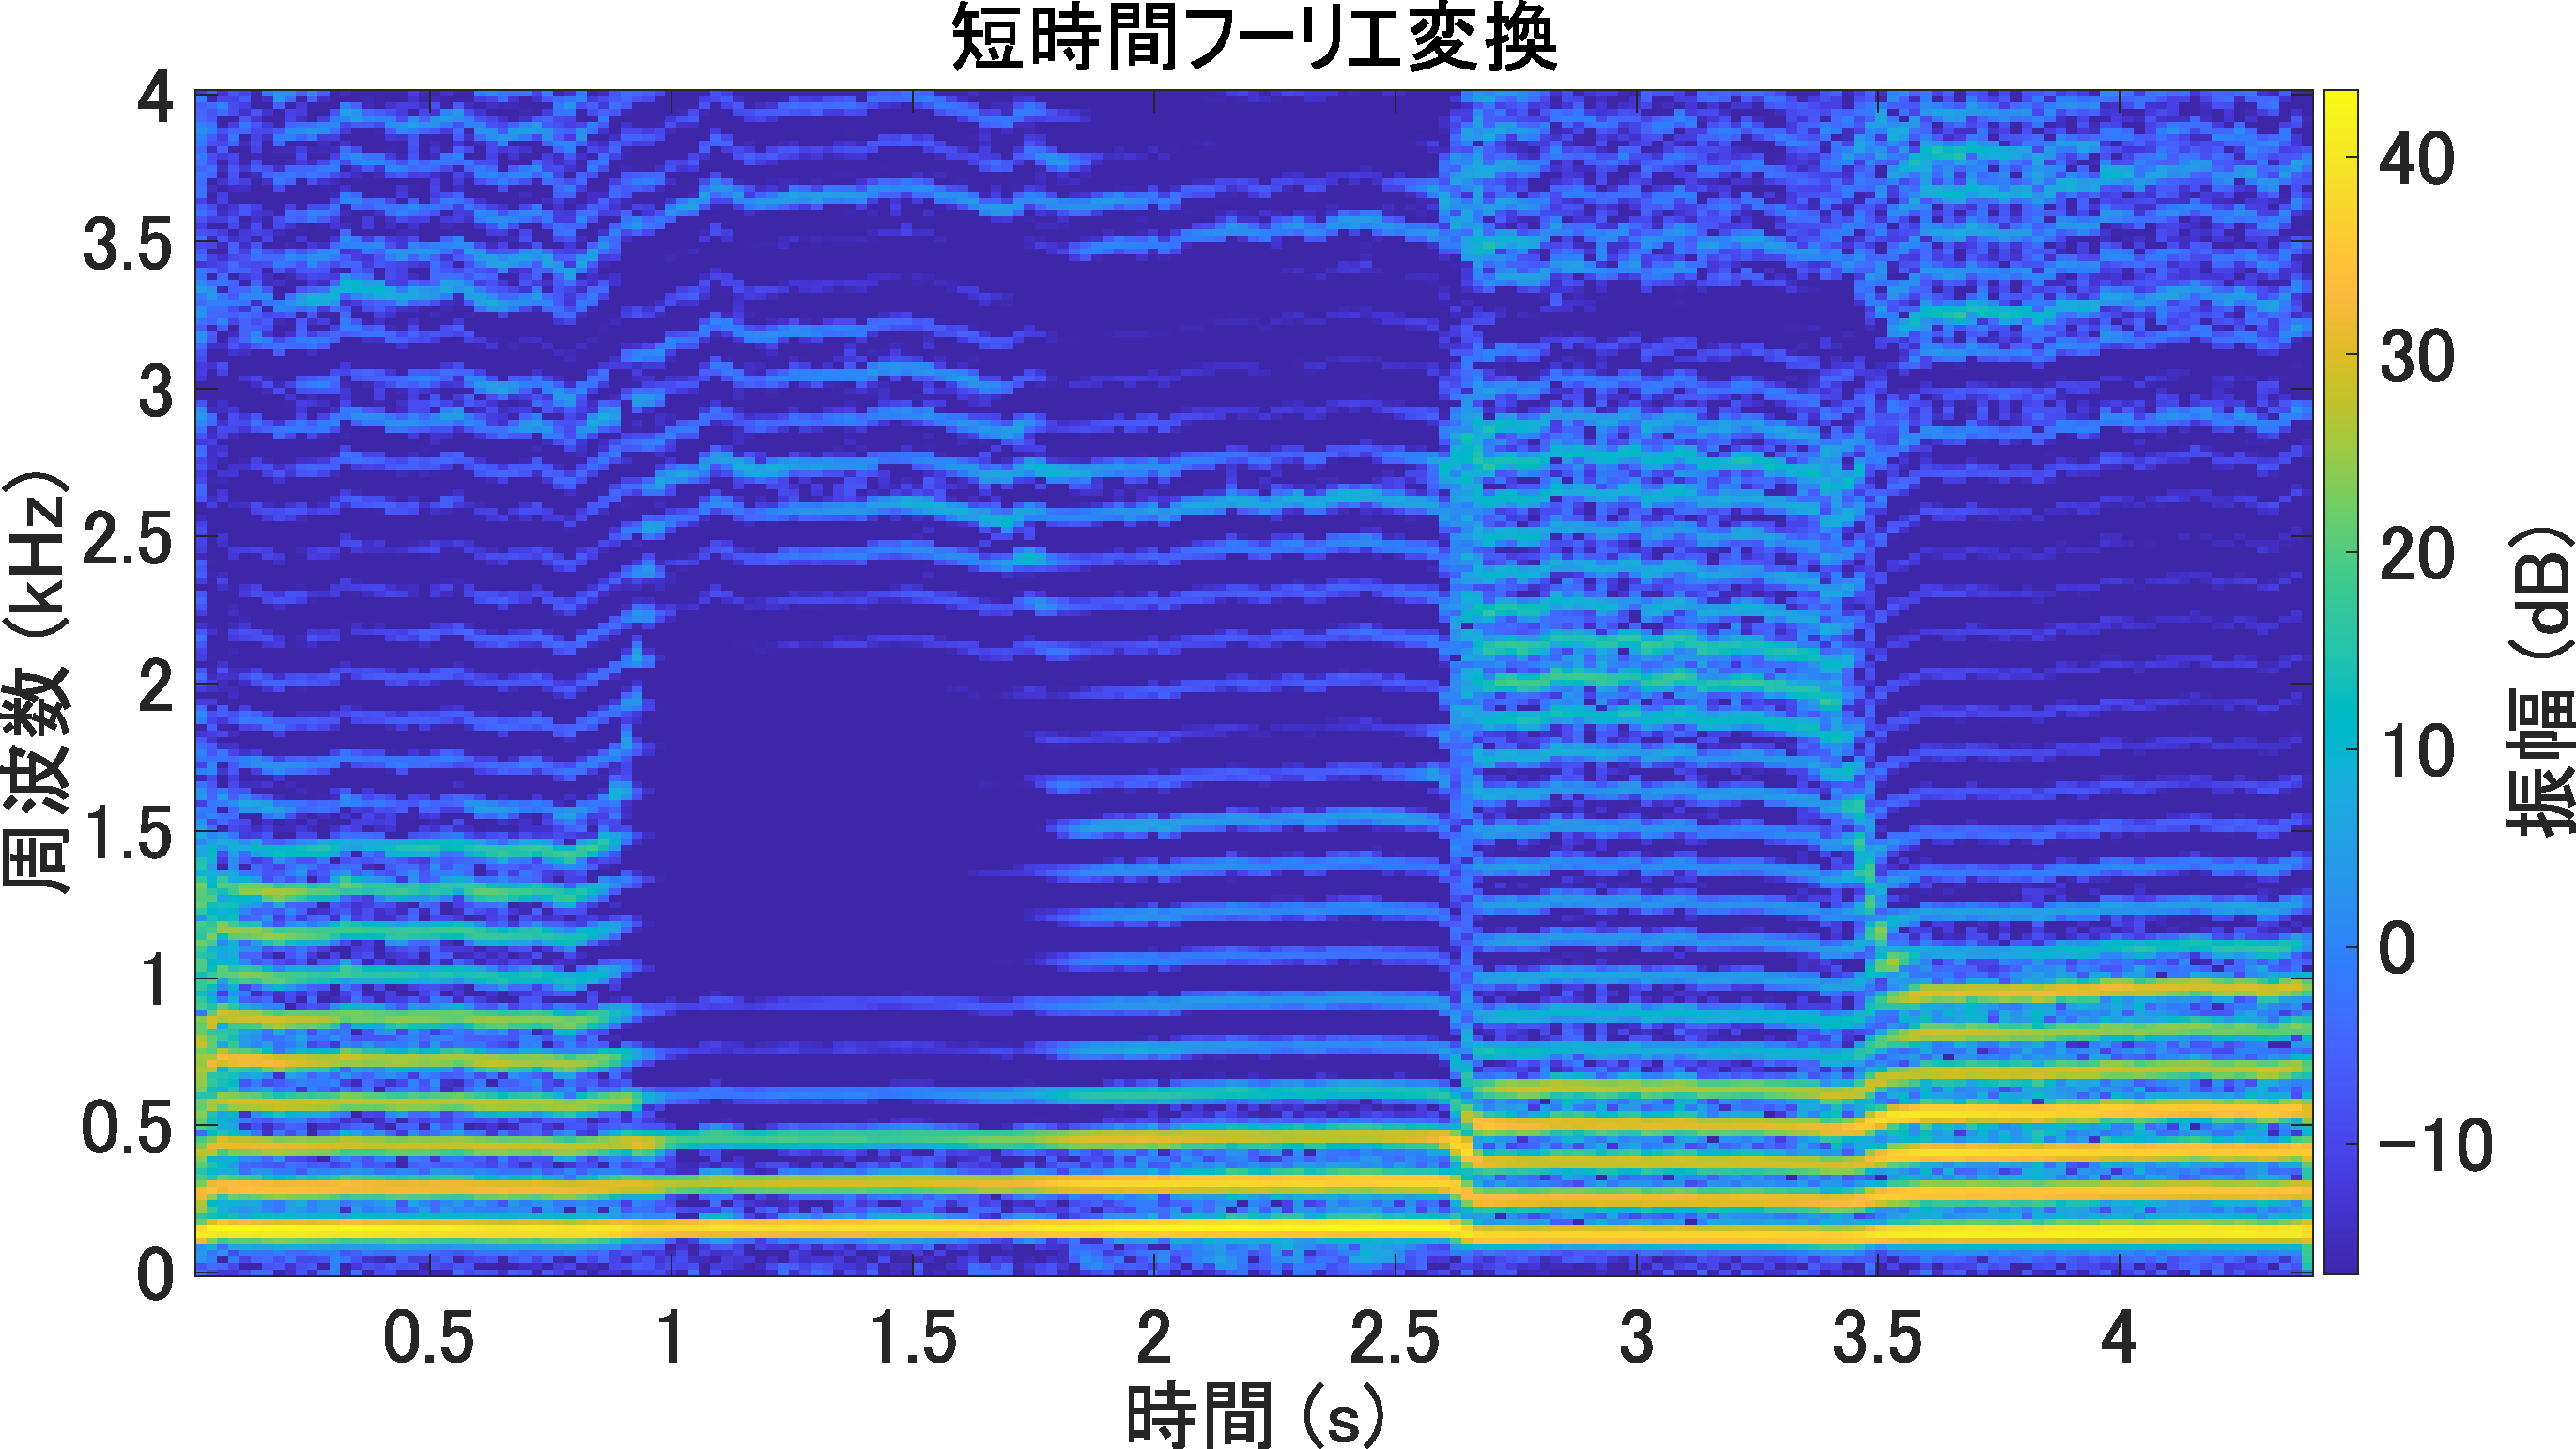
\includegraphics[width=9cm]{./figure/spectrogram.pdf}
    \caption{「あいうえお」の\(20\log_{10}\abs{\STFT x(k,\Omega)}\)の様子}
  \end{figure}
\end{frame}

\begin{frame}
  \frametitle{\secname :\subsecname}
  さきほどの図から,ある時刻\(k\)における短時間フーリエ変換は
  「緩やかで非周期的な変動」と「激しく周期的な変動」を併せ持つことが分かる.
  前者のことを\termdef{スペクトル包絡}という.

  後者は声の高さに起因する成分だから,前者は声から「声の高さ」の影響を取り除いたときに
  残る成分である.より大雑把に言うと,スペクトル包絡は声の「音色」に相当するパラメータである.
\end{frame}

\begin{frame}
  \frametitle{\secname :\subsecname}
  それでは,スペクトル包絡はどうやって算出すればよいのだろう? 有名かつ古典的な手法として,次の2つが知られている.
  \begin{itemize}
    \item 線形予測分析
    \item ケプストラム法
  \end{itemize}
\end{frame}

\begin{frame}
  \frametitle{\secname :\subsecname}
  大雑把に2つの概要を述べて,この発表を終わりとすることにしよう\footnote{\cite{takamichi2015,morise2018}により詳しい記述がある.}.
  線形予測分析では,音声が\(p\)次の\termdef{自己回帰過程}
  \[
    x[n] = \sum_{i=1}^p\phi_ix[n-i]+\epsilon_n
    \quad\text{(\(\epsilon_n\)はホワイトノイズ)}
  \]
  にしたがうと仮定し,\(\phi_1,\dots,\phi_p\)を推定することで,
  信号のスペクトル包絡を推定する.

  一方,ケプストラム法では,\cref{figure:spectre}のグラフを平滑化する(山と谷を均す)ことでスペクトル包絡を求める.
\end{frame}

\section{補遺}
\subsection{離散フーリエ変換}
\begin{frame}
  \frametitle{\secname :\subsecname}
  \begin{block}{\subsecname}
    ここでは線形代数の応用として,離散フーリエ変換について紹介する(短時間フーリエ変換は「離散フーリエ変換を繰り返し行うこと」と解釈できる).

    \begin{definition}[離散フーリエ変換]
      有限長の複素数列\(\vb{x}=\trps{\inlinevec{x_0 & \cdots & x_{N-1}}}\)に対し,
      \(\vb{x}\)の\termdef{離散フーリエ変換}\(\vb{X}=\trps{\inlinevec{X_0 & \cdots & X_{N-1}}}\in\numset{C}^N\)を
      \[
        X_n = \frac{1}{\sqrt{N}}\sum_{k=0}^{N-1}x_ke^{-i(n\Delta\Omega)k}
        \quad\text{(\(\Delta\Omega=2\pi/N\))}
      \]
      により定義する.
    \end{definition}
  \end{block}
\end{frame}

\begin{frame}
  \frametitle{\secname :\subsecname}
  以下では,離散フーリエ変換の意味づけを与える.信号\(\Set{x_n}\)が周期\(N\)の周期数列なら,
  \(\Set{x_n}\)はベクトル\(\vb{x}=\trps{\inlinevec{x_0 & \cdots & x_{N-1}}}\)と
  1対1に対応する.つまり,\(\Set{x_n}\)について調べるには,\(\vb{x}\)について調べれば十分である.

  さて
  \[
    \vb{w}_n = \frac{1}{\sqrt{N}}\trps{\begin{bmatrix}e^{i(n\Delta\Omega)0} & \cdots & e^{i(n\Delta\Omega)(N-1)}\end{bmatrix}}
    \quad\text{(\(\Delta\Omega=2\pi/N\))}
  \]
  とおくと,\impact{\(\basis{B}=\Set{\vb{w}_0,\dots,\vb{w}_{N-1}}\)は\(\numset{C}^N\)の正規直交基底になる}.
  ということは,\(\vb{x}=X_0\vb{w}_0+\dots+X_{N-1}\vb{w}_{N-1}\)
  を満たす\(X_0,\dots,X_{N-1}\in\numset{C}\)は一意に定まる.
\end{frame}

\begin{frame}
  \frametitle{\secname :\subsecname}
  \(X_n\)を求めよう.\(\basis{B}\)は正規直交基底だから
  \begin{align*}
    \innerp{\vb{x}}{\vb{w}_n} &= X_0\innerp{\vb{w}_0}{\vb{w}_n}+\dots+X_{N-1}\innerp{\vb{w}_{N-1}}{\vb{w}_n} \\
    &= \cancelto{0}{0X_0+\dots}+1X_n+\cancelto{0}{\dots+0X_{N-1}}
  \end{align*}
  である.\(\innerp{\vb{x}}{\vb{w}_n}\)を\(\sum\)によって書けば,次のようになる.
  \[
    X_n = \frac{1}{\sqrt{N}}\sum_{k=0}^{N-1}x_ke^{-i(n\Delta\Omega)k}
  \]

  これは離散フーリエ変換に他ならない.つまり,\impact{離散フーリエ変換はベクトルの基底を取り換える操作}と捉えられる.
\end{frame}

\subsection{フーリエ変換}
\begin{frame}
  \frametitle{\secname :\subsecname}
  \begin{block}{\subsecname}
    \(\omega\in\numset{R}\)を固定する.
    離散信号\(e^{i\Omega n}\)は,連続信号\(e^{i\omega t}\)を標本化して得られたものだとする.
  
    \(x[n]=x(n\Delta t)\)という式を思い出すと,\(e^{i\Omega n}=e^{i\omega n\Delta t}\)でなければならない.
    したがって,\(\Omega\)と\(\omega\)の間には\(\Omega=\omega\Delta t\)という関係がある.      
  \end{block}
\end{frame}

\begin{frame}
  \frametitle{\secname :\subsecname}
  \begin{columns}
    \begin{column}{0.6\textwidth}
      \[
        X(\omega\Delta t) = \sum_{n=-\infty}^\infty x(n\Delta t)e^{-i(\omega\Delta t)n}
      \]
      であるから,\(\Delta t\)を掛けて極限をとれば次のようになる.
      \begin{align*}
        &X(\omega\Delta t)\Delta t \\
        &= \sum_{n=-\infty}^\infty x(n\Delta t)e^{-i\omega n\Delta t}\Delta t \\
        &\to \underbrace{\int_{-\infty}^\infty x(t)e^{-i\omega t}\intd{t}}_{\text{\(\ft x(\omega)\)とおく}} \plimas{\Delta t\to +0}
      \end{align*}
    \end{column}
    \begin{column}{0.4\textwidth}
      \begin{figure}
        \centering
        \begin{tikzpicture}
          \begin{axis}[width=\figurewidth,axis lines=middle,axis line style={->},xmin=-0.1,xmax=1.1,xtick=\empty,ytick=\empty,cycle list name=linestyles,legend columns=3,legend style={at={(0.5,1.03)},anchor=south}]
            \node [above] at (axis cs:0.2,0) {\(\scriptstyle 1\Delta t\)};
            \node [above] at (axis cs:0.4,0) {\(\scriptstyle 2\Delta t\)};
            \node [above] at (axis cs:0.6,0) {\(\scriptstyle 3\Delta t\)};
            \addplot+ [black,smooth,samples=100,domain=-0.2:1.2] {(5*x^3-3*x)/2-0.2};
            \addplot+ [black,ybar interval,samples=8,domain=-0.2:1.2] {(5*x^3-3*x)/2-0.2};
            \addlegendentry{\(\scriptstyle\ft x(\omega)\)};
            \addlegendentry{\(\scriptstyle X(\omega\Delta t)\Delta t\)};
          \end{axis}
        \end{tikzpicture}
        \caption{\(X(\omega\Delta t)\Delta t\to\ft x(\omega)\plimas{\Delta t\to +0}\)のイメージ図}
      \end{figure}
    \end{column}
  \end{columns}
\end{frame}

\begin{frame}
  \frametitle{\secname :\subsecname}
  \begin{columns}
    \begin{column}{0.6\textwidth}
      \begin{definition}[フーリエ変換]
        関数\(x(t)\)に対し
        \[
          \ft x(\omega) = \int_{-\infty}^\infty x(t)e^{-i\omega t}\intd{t}
        \]
        で定義される関数\(\ft x(\omega)\)を,\(x(t)\)の\termdef{フーリエ変換}という.
      \end{definition}
    
      各\(\omega\)について,\(\ft x(\omega)\)は\(x(t)\)に含まれる\(e^{i\omega t}\)という関数の
      「振幅」と「位相」を表している.    
    \end{column}
    \begin{column}{0.4\textwidth}
      \begin{figure}
        \centering
        \begin{tikzpicture}
          \begin{axis}[width=\figurewidth,ticks=none,axis lines=center,xlabel={\(\scriptstyle t\)}]
            \draw [->] (axis cs:0,0,0) -- (axis cs:0,{cos(120)},{sin(120)});
            \addplot3 [domain=0:18,samples=100,samples y=1] ({x},{cos(deg(x)+120)},{sin(deg(x)+120)});
          \end{axis}
        \end{tikzpicture}
        \caption{\(Ae^{i(\omega t+\phi)}\)のグラフ(時間軸と直交する平面は複素平面)}
      \end{figure}
    \end{column}
  \end{columns}
\end{frame}

\section*{参考文献}
\begin{frame}[allowframebreaks]
  \frametitle{参考文献}
  \beamertemplatetextbibitems
  \bibliographystyle{jplain}
  \bibliography{index}
\end{frame}

\end{document}
